\subsection{Technical description}
%The system can be described as a Classroom Response System (CRS) in the sense that it's a system made for polling and gathering responses in a classroom.


The following section will provide a technical description of the system and how it's made. The section will include examples of code describing different parts of the system and an outline of the structure of the project and describe how we store data. Furthermore, we will include descriptions of different parts of the system and the libraries and third-parties they rely on. In the end, we will explain how the system is deployed to the web.

Before describing the system, we will give a brief explanation of the technologies behind.

The system is implemented as a web application using the Python programming language and the Django web framework. For data storage we are using a MySQL database.
For development purposes we are using \texttt{virtualenv}, a plugin that allows virtual python environments. The following sections will describe all of these parts and a few more in detail below.

\subsubsection*{Django web framework}
We have chosen the Django web framework to build the system. Django is an open-source web framework build with Python. We are using Django version 1.9.1 which was the latest release when we started developing the system.

Django uses the \emph{Model-View-Controller} (\emph{MVC}) pattern to structure projects. %\emph{Models} are the objects in the project. 
Models are translated into tables in the database, so writing a model is similar to creating tables in a SQL database. E.g., the following model from CRSFIT defines \emph{Room}: 

\begin{lstlisting}[caption=The Room Class, label=lst:room-class]
class Room(models.Model):
    owner = models.ForeignKey(User)
    title = models.CharField(max_length=200)
    date_time = models.DateTimeField(auto_now_add=True)
    updated_at = models.DateTimeField(auto_now=True)
    
    def function_name(self):
        # do stuff
\end{lstlisting}




\emph{Views} are defined in the \texttt{views.py} file within each Django app, and corresponds to the \texttt{Controller} in the MVC pattern. Views can specify which \emph{template} should be rendered and what context is provided in the template. The only requirement for each view, is that it must return a HTTP response. Often the view also checks several things such as if the request is allowed to retrieve the data from the view or not. Here's an example of the \texttt{room\_edit} view:

\begin{lstlisting}[caption=The Room edit method, label=lst:room-edit-method]
def room_edit(request, room):
    room = get_object_or_404(Room, pk=room)
    if not room.owner == request.user:
        return redirect(room)
    context = {'room': room, 'form': VoteRoomForm(instance=room)}
    return render(request, 'vote/room_edit.html', context)
\end{lstlisting}
This view also ensures that the room exists through the \texttt{get\_object\_or\_404()} method, and whether or not the requester is the owner of the room. If the requester is not the owner, then he is redirected back to the room, otherwise he is shown the edit page for it. The provided context in the template can be found in the context variable. The context is the data that is passed along to the view when it is rendered. In this case, the room object and a \texttt{VoteRoomForm}. The form is created with the instance set to that room. This means that whatever data is in the room object, is bound to the \texttt{VoteRoomForm}. When the view is rendered, all the data that is stored for that room, is automatically shown in the corresponding form fields. 

Templates is what gets rendered and shown in the browser. The templates in Django corresponds to views in the MVC pattern. Templates are mainly regular HTML. Within a template it's possible to use Django's template language to access the context provided by the view.

A url pattern is also found within each Django app. It's defined in the \texttt{urls.py} file where a regular expression is matching and directing URL requests to different views. Parts of an \texttt{url.py} file can be seen here:

\begin{lstlisting}[caption=URL patterns from the vote app, label=lst:urlpatterns]
urlpatterns = [
    # ROOM
    url(r'^room/create/$', views.CreateRoomView.as_view(), name='room_create'),
    url(r'^room/(?P<pk>[0-9]+)/$', views.RoomDetailView.as_view(), name='room_detail'),
    url(r'^room/(?P<room>[0-9]+)/edit/$', views.room_edit, name='room_edit'),
    url(r'^room/(?P<room>[0-9]+)/delete/$', views.room_delete, name='room_delete'),
    ...
    ]
\end{lstlisting}
Each requested URL from the system is being matched with one of these regular expressions which in return directs to a \emph{view} method. The parameters in each view method is passed along from the url, for example where the URL says \texttt{?P<room>[0-9]+}, the regular expression matches any number combination with room id's, and the method will get a room id passed along.

% Beside using many of Django's features, we also do use an amount of external Python libraries. A full list can be found in \texttt{requirements.txt}.

\subsubsection*{Data storage}
We have chosen a MySQL database for our data storage. Within Django's settings file for the project (\texttt{settings.py} in the main app) we specify which drivers to use and login credentials to the database. Django handles all the connections, writing and reading to and from the database using Djangos own ORM (Object-relational mapping). Every time an object is created, changed or deleted (a user, a question, an answer etc.) Django handles transactions and communication with the database. The models specified in each app handles all the direct database interaction, exposing only methods needed to perform these actions. This also enables us to easily handle other databases like PostgreSQL, since we are only being specific to Django, and not to any specific database.

We could have chosen a different database for the system such as PostgreSQL. This would only require us to add a different database to the before mentioned settings, tell Django to migrate and remove the old database from the settings when done. This is convenient for changing the database at a later point if it should be necessary. The process of moving the data stored in the database, is still a manual process though.

%This makes a third party ORM unnecessary. An ORM is typically a third party service which is sometimes paid for and takes time to integrate with the chosen framework. A short discussion of this problem can be found in the article by \citeA{johnson2005j2ee} where he highlights some of the history of Java's integration with ORMs.

\subsubsection*{Caching}
To prevent our database from being hit too often we have added caching to the site. In this case we are using Memcached\footnote{\url{https://memcached.org/}}. We are primarily caching the static pages on the site, and the search results. This way common search queries will not hit the database so often. For testing purposes this is not overly important, but we do wish to have a robust and scalable infrastructure.

\subsubsection*{Python, virtualenv and external packages}
For development we are using a virtual environment created with \texttt{virtualenv} to handle the required packages and their versioning for the project. The environment also specifies which version of Python is used (3.5.1). The environment is only active when it's activated, enabling us to use any version of Python we want. When it's deactivated the systems default is used. The packages are only installed within the environment and will not be available on the system when the environment is deactivated which makes package management easy and convenient.

We've used a few external Python packages for creating this project, which can be found in the \texttt{requirements.txt} file. Within this file we can specify which version of each package we want to use when installing a package. An omitted version number means the newest version is installed. The full list of packages is shown in listing \ref{lst:requirements}.

\begin{lstlisting}[caption=The requirements.txt file. , label=lst:requirements]
    mysqlclient
    django==1.9.1
    django-environ==0.4.0
    django-widget-tweaks
    django-mailgun
    django-super-inlines
    pusher
    bleach
    django_compressor
    short_url
    python-memcached
\end{lstlisting}

All packages are installed by running the command \texttt{pip install -r requirements.txt} within the virtual environment. A detailed description of selected packages are given in this section according to where in the system they are used.

\subsubsection*{Project Structure}
The structure of the project can be seen below. Folders are indicated by a trailing slash. The project itself is called CRS and is located at the root of the structure. All the folders shown in the CRS folder are Django applications (apps). An app in Django-terminology is a separate part of the system, that \emph{"... describes a Python package that provides some set of features."}\footnote{Retrieved on 2016-04-01, \url{https://docs.djangoproject.com/en/1.9/ref/applications/\#projects-and-applications}}. The vote folder is expanded to show the underlying structure, as an example of an application structure.

\begin{figure}[H]
    \dirtree{%
        .1 CRS.
            .2 authentication/.
            .2 dashboard/.
            .2 home/.
            .2 main/.
            .2 vote/.
                .3 \_\_pycache\_\_/.
                .3 migrations/.
                .3 static/.
                .3 templatetags/.
                .3 templates/.
                .3 \_\_init\_\_.py.
                .3 admin.py.
                .3 apps.py.
                .3 forms.py.
                .3 models.py.
                .3 tests.py.
                .3 urls.py.
                .3 utils.py.
                .3 views.py.
            .2 README.md.
            .2 manage.py.
            .2 requirements.txt.
    }
    \caption{The Django project structure}
    \label{fig:project-structure}
\end{figure}

The CRS project consists of five applications. \texttt{authentication}, \texttt{dashboard}, \texttt{home}, \texttt{main} and \texttt{vote}. Each is responsible for their own part of the CRS service, and their names are supposed to be self explanatory to a certain extend, after a proper introduction.

% Basic feature
\subsubsection*{Authentication}
The \texttt{authentication} app is responsible for all the application's authentication logic. This includes logging in users, logging them out, signing up and resetting passwords.

It's necessary to register and sign in with personal credentials (username and password) in order to use the system. Anyone can register for an account from the frontpage or from the login page.

We use Django's build in user authentication to manage all aspects of users in the system. This includes registering users, signing in, resetting passwords - all the time consuming but critical features usually wanted in a system involving users. Furthermore, Django provides an easy to use protection against cross site request forgeries which protects users from getting their credentials stolen or from being session hijacked.

Since we want to register users with an email, we have added a field to our custom user creation form. The \texttt{User} model already includes an email field, so it's only necessary to add the form input field. This is done by adding the field as shown in listing \ref{lst:custom-user-creation-form-class} on line 2, and then overriding the save method to include it as shown in line 9.


\begin{lstlisting}[caption=CustomUserCreationForm class, label=lst:custom-user-creation-form-class]
class CustomUserCreationForm(UserCreationForm):
    email = EmailField(label=_("Email address"),
                       required=True, 
                       help_text=_("Required."))
    class Meta:
        model = User
        fields = ("username", "email", "password1", "password2")

    def save(self, commit=True):
        user = super(CustomUserCreationForm, self).save(commit=False)
        user.email = self.cleaned_data["email"]
        if commit:
            user.save()
        return user
\end{lstlisting}

The email is crucial for resetting passwords, otherwise the account will be lost if a user forgets his/her password. The whole process is handled by Django as long as we provide a email back-end which is specified in the \texttt{settings.py} file found in the main app. In order to send emails we use the external service Mailgun\footnote{Retrieved on 2016-04-04: \url{https://www.mailgun.com/}}, which sends email on behalf of the system. Whenever a user requests to reset a password, an email with a unique link is sent to the users email address. The link is automatically created by Django and could look like this:  \texttt{.../authentication/reset/MTY/4as-663c1494cfc7b061c25d/}. This links redirects to a page from where the user can enter a new password.

\subsubsection*{Dashboard}
The \texttt{dashboard} app is responsible for handling the users dashboard. When a user logs in, they are presented with a personal dashboard that shows a variety of information, relevant for that user.
The dashboard contains information about which rooms the user is subscribed to and information about the rooms the user owns. It's possible to create new rooms directly from the dashboard. The search endpoint is also registered within the dashboard app. Searching is added as a convenience feature for the first iteration of the project and is not meant for actual production use. A full text search feature using a search engine like Solr\footnote{\url{http://lucene.apache.org/solr/}} or Elasticsearch\footnote{\url{https://www.elastic.co/products/elasticsearch}} would be preferable, but since it will not add any direct value to answering our research question, it is currently implemented as a simple database lookup on room names for now.

\subsubsection*{Home} %\todo{Tilføj mere lækkert til home beskrivelsen}
The \texttt{home} app handles static pages like the front page and the user profile pages.
All pages related to the home application is located within the home app. Also, the short-URL feature found in groups is handled from here. Examples of common pages that could be created here is an 'About Us' page, an FAQ etc., but since we are only providing the most necessary features pages like that has not been included.

\subsubsection*{Main}
The \texttt{main} app is special, as it is the \emph{root} app in the project. It contains the \texttt{settings.py} file, which is global for all applications. It is also where generic templates are located, such as the \texttt{base.html} file, that contains the main html structure of all pages throughout the site. Here we are able to include static asset files such as JavaScript, CSS and metatags that should be included on every page. Templates such as navigation bars and logic for showing messages to the user is located here as well.

\subsubsection*{Vote}
The \texttt{vote} app is the most comprehensive app in the project. It holds all the logic for creating questions, registering votes, showing responses etc. Except for the creation of rooms, every url that you can visit in the vote app requires a room primary key. In listing \ref{lst:urlpattern-for-room-edit} the primary key is the room id. The id is expressed as a regular expression with the name room, as specified within the brackets \texttt{<room>}. The name here does not matter and could be anything, but for the sake of readability we have chosen room.

\begin{lstlisting}[caption=URL Pattern for Room Edit, label=lst:urlpattern-for-room-edit]
url(r'^room/(?P<room>[0-9]+)/edit/$', views.room_edit, name='room_edit')
\end{lstlisting}

\subsubsection*{Models}
The rooms (and any other entity that we have defined here) is expressed as a Django Model.  
The models can have fields defined, as well as methods. The room example in listing \ref{lst:room-model} has the fields owner, title, \texttt{date\_time} and \texttt{updated\_at} and some convenience methods.


\begin{lstlisting}[caption=The Room model, label=lst:room-model]
class Room(models.Model):
    owner = models.ForeignKey(User, on_delete=models.CASCADE)
    title = models.CharField(max_length=200)
    date_time = models.DateTimeField(auto_now_add=True)
    updated_at = models.DateTimeField(auto_now=True)

    class Meta:
        unique_together = ('owner', 'title')

    def get_absolute_url(self):
        return reverse('room_detail', kwargs={'pk': self.pk})

    def has_questiongroups(self):
        return len(self.questiongroup_set.all()) > 0

    def has_open_questiongroups(self):
        for questiongroup in self.questiongroup_set.all():
            if questiongroup.is_open:
                return True
        return False

    def total_subscribers(self):
        return len(self.subscription_set.all())

    def __str__(self):
        return self.title
\end{lstlisting}


The model in listing \ref{lst:room-model} inherits from Django's \texttt{Model} class. Each field above corresponds to a column in the database. Foreign keys are represented as other models. As seen above, the \texttt{Room} model belongs to one \texttt{User} model, which is the owner of that room. 
It's possible to define functions which belongs to a specific model. The Room model has several functions. One of these functions, \texttt{def total\_subscribers(self)}, returns the number of subscribers and looks like this:

\begin{lstlisting}[caption=The total subscribers method, label=lst:total-subscribers-method]
def total_subscribers(self):
    return len(self.subscription_set.all())
\end{lstlisting}
This way of reasoning is simple to follow and puts logic belonging to a specific model right where the model is. The method as it is implemented above, retreieves the Room's subscriptions in an array, and uses the \texttt{len()} Python method to count the length of it. Another way of doing this, more closely related to Django, is by calling the \texttt{count()} method like this \texttt{return self.subscription\_set.count()}.

%The owner is defined as a foreign key and represents a User relationship. In this case, a Room must belong to a User. 
The \texttt{date\_time} and \texttt{updated\_at} fields are automatically updated with the \texttt{auto\_now\_add} and \texttt{auto\_now} attributes set to \texttt{True}. The model also has a \texttt{Meta} class defined. In this case it only defines the unique database keys, but it could contain more information.

\subsubsection*{Input sanitation}
The voting app contains a lot of user input. Each room has a name that is created by the user. The groups, questions and answers also relies heavily on user generated input. To prevent users from creating malicious input, we are sanitizing everything using Bleach on the server side. Bleach is a \emph{"... whitelist-based HTML sanitizing library that escapes or strips markup and attributes."}\footnote{Retrieved on 2016-04-04\url{https://bleach.readthedocs.org/en/latest/}}. We are then capable of sanitizing input by calling the \texttt{clean} method on a Bleach instance. An example of using bleach in the project, can be found in the \texttt{question\_answer\_create} method as seen in listing \ref{lst:bleach}:

\begin{lstlisting}[caption=Using Bleach to sanitize input, label=lst:bleach]
bleach.clean(new_question.question_text, tags=ALLOWED_TAGS)
\end{lstlisting}

The \texttt{ALLOWED\_TAGS} is the whitelist consisting of an array, that defines which tags are allowed and which are to be stripped/sanitized away. Since the system supports code input, it is important that the user is able to input fx. \texttt{<script>} tags. Obviously we do not want any of the JavaScript input to be executed when the page loads, and Bleach helps us do this, by escaping the tags that are not white listed.
The current version of the CRSFIT application does not have any client side validation. The server side validation is most important for keeping our data safe, where the client side validation is good for usability and potentially lowering the amount of invalid data posted to the server.

\subsubsection*{WYSIWYG editor}
We have implemented TinyMCE\footnote{\url{https://www.tinymce.com/}} in the system, a \emph{What You See Is What You Get}-editor. This is done in order to provide a familiar way of editing text. Using TinyMCE we can add custom features like the \texttt{PRE} button to mark text as code. See figure \ref{fig:tinymce} for a view of the editor, where a question has been added with text formated as code in the middle.

\begin{figure}[H]
\capstart
	\centering
		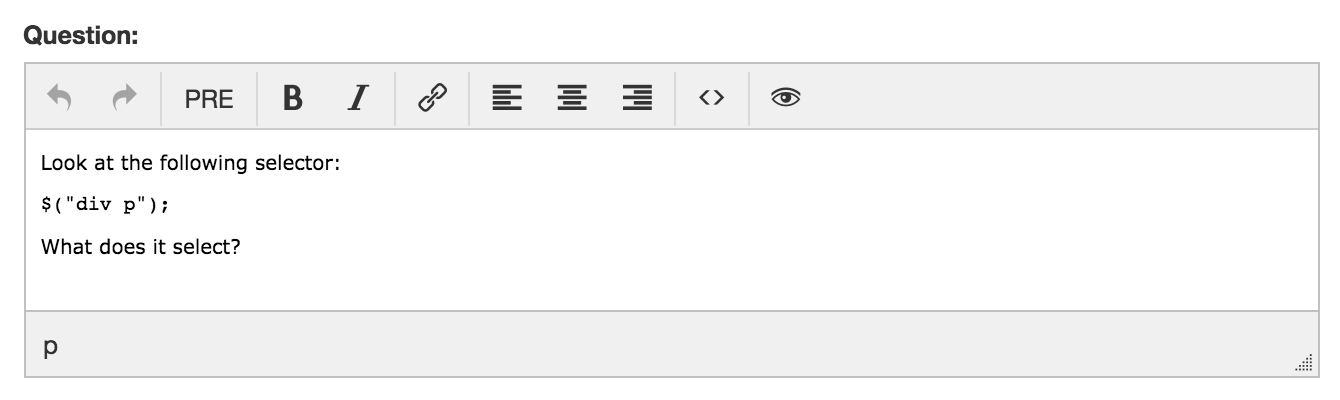
\includegraphics[width=\textwidth]{tinymce.png}
	\caption[TinyMCE]{TinyMCE editor as implemented in CRSFIT.}\label{fig:tinymce}
\end{figure}

\subsubsection*{Short URL}
To access a group directly it is necessary to know the URL. As a convenience, a url shortening feature is added to all groups using the \texttt{short\_url} library\footnote{\url{https://pypi.python.org/pypi/short_url}}. The url is not stored as persistent data, but simply generated on the fly. When a user makes a GET request to one of the shortened URL's the following method is hit.

\begin{lstlisting}[caption=The URL redirect method, label=lst:url-redirect]
@login_required
def url_redirect(request, short):
    group_id = short_url.decode_url(short)
    group = get_object_or_404(QuestionGroup, pk=group_id)
    return redirect(group)
\end{lstlisting}

The \texttt{short} parameter is the short key that is generated when a group is requested. Since we can decode it, it's possible to retrieve the group and redirect to it as shown in listing \ref{lst:url-redirect}. The url-shortening feature is provided as a convenience to allow students to easily access groups. The intention here was to make it as easy as possible to access a group of questions, to avoid possible confusion while navigating the interface.

\subsubsection*{Live updates}
Whenever someone answers a question the response can be seen live by the owner of the question at \texttt{.../question/<question-number>/responses/}. The graph will automatically update and display the current result. In order to show live updates we use Pusher. Pusher is a service for sending and receiving live data easily\footnote{Retrieved on 2016-04-04 \url{https://pusher.com/}}.
In order to use Pusher we create a channel to which we subscribe and bind an event to. This can be seen in \texttt{push.js} found in the vote app. The event that triggers Pusher is whenever someone answers a question. To tell Pusher, that there's a new event we trigger Pusher from the \texttt{answer\_response} view and provide it with the relevant data:

\begin{lstlisting}[caption=Selected parts of the answer\_response view, label=lst:answer_response]
        ...
        myData = {
            'total_responses': question_obj.total_responses(),
            'labels': [a.answer_text for a in answer_set],
            'series': [a.number_of_responses() for a in answer_set]
        }
        event = "response-%s%s%s" % (room, questiongroup, question)
        get_pusher().trigger('crs', event, {'data': myData})
    return redirect(qg)
\end{lstlisting}

The trigger at line 8 in listing \ref{lst:answer_response}, is where the view tells Pusher that there's a new event. From here, Pusher tells all subscribers of the corresponding channel, \texttt{crs}, that there's a new event which we can then handle. The event name should be unique, otherwise everybody will receive the same data. To ensure uniqueness we simply join each primary key for room, questiongroup and question into a string. This way we can separate responses from each other and ensure that graphs are not updated with data from other questions.
In \texttt{push.js} we do the following to subscribe and handle the events sent by the view:

\begin{lstlisting}[caption=Selected parts of push.js, label=lst:push.js]
var channel = pusher.subscribe('crs');
var event = $("#event:hidden").val();
channel.bind(event, function(data) {
    divs = $(".answer-box");
    divs.each(function(index, value){
        var answerId = parseInt($(value).attr('id'));
        var answer_count = data.data[answerId] ? data.data[answerId].answer_count : 0;
        $(value).text(answer_count);
    });
    $("#response-count").text(data.data.total_responses);
    chart.update(data.data);
});
\end{lstlisting}
The code in listing \ref{lst:push.js} subscribes to events on the channel named \texttt{crs} and handles updates to the response page by getting the data from the event and displaying it in the chart besides updating the number of total responses.


\subsubsection*{Deployment}
%\todo{Vi skal da have en oversigt over hvordan det er sat op på amazon med database server, S3 for static files osv. Tænkte jeg godt på :) Det kan vi jo sagtens, så kan vi bruge lidt fra Scalability faget OMG}

For deployment of the system we have chosen a 3-tier architecture. This consists of one web server, one media server and one database server as shown in figure \ref{fig:3-tier}. 

\begin{figure}[H]
\capstart
	\centering
		\includegraphics[width=7.5cm]{n-tier-diagram.png}
	\caption[]{The 3-tier architecture \label{fig:3-tier}}
\end{figure}

The web server is responsible for hosting Django and all the dynamic content, such as the HTML files. The media server is used to host static files, such as CSS, JavaScript and images. The database is hosted on a server of it's own, this allows us to easily add more web servers for scaling if needed.

The system is hosted using Amazon Web Services (AWS)\footnote{\url{https://aws.amazon.com/}}. The web server is an EC2 instance running Ubuntu 14.04 with Apache2 and Django installed. The Apache2 web server is installed with the \texttt{mod\_wsgi}\footnote{\url{https://modwsgi.readthedocs.io/en/develop/}} mod, to support Python WSGI applications.

The media server is an Amazon S3 bucket, containing all the static files. For the database, we are running an Amazon Relational Database Service (RDS) instance. Using RDS have several advantages. First, all data is separated from our web server. This makes horizontal scaling of the web servers very easy, since we simply need to add another copy of our EC2 instance to the cluster and add a load balancer in front of that, as shown in figure \ref{fig:n-tier}.

\begin{figure}[H]
\capstart
	\centering
		\includegraphics[width=9.5cm]{2-n-tier-diagram.png}
	\caption[]{The n-tier architecture \label{fig:n-tier}}
\end{figure}

Secondly vertical scaling is possible, since it is only a question of telling the EC2 instance to add more RAM, bigger CPU or whatever might be needed to gain more power \cite[p.~204]{henderson2006building}.

It would be ideal to run the n-tier setup from the beginning, since the 3-tier setup has one major fault, if one server fails, everything fails. There is no redundancy available, so we are vulnerable to potential full system failure. Even the n-tier setup shown in figure \ref{fig:n-tier} is not redundant enough, since there's still only one media server, and one database server. That means that even though we might be scalable in the terms of larger amounts of traffic, we are still vulnerable to system failures. If we needed to upgrade a server, only having one of each would possibly result in downtime. Having more would enable us to upgrade one node at a time, ensuring no downtime at all.

Currently memcached is running on the EC2 instance. This is not a viable solution if we were to scale the webservers horizontally. Depending on which server you get redirected to by the loadbalancer, potential cache inconsistency could occur. This is however easily fixed, by adding another server handling all the caching. We have added caching to prove a point, and are aware that this setup could be improved. The addition of a separate cache server however costs money by the hour, and has not been included.

% The most preferable mode of redundancy 
Since we are only using this for demo purposes, we have gone with the 3-tier setup as a minimum working solution, keeping the n-tier setup as a possible future architecture for a real production environment.






\subsection{Summary}
In the sections above we have described CRSFIT in detail. It's features, how it is developed, the tools used and the deployment process. To summarize all the features, compared to section  \ref{sec:competitor-overview}, we have added CRSFIT to the overview as shown in table \ref{tab:overview-2}.


\begin{landscape}
\thispagestyle{empty}
    \begin{center}
        \begin{table}[H]
            \begin{tabularx}{\paperwidth}{ |X|X|X|X|X|X|X|X|X| } 
             \hline
                 & Web \newline Software \newline Hardware based & Multiple question types & Multiline support & Mathematical notation & Source code notation & Supports image upload as questions & Timed questions/auto closing questions & Payment model \\ \hline
                 
              Kahoot                & Web   & No    & No    & \cellcolor{red!25}No    & \cellcolor{red!25}No    & Yes   & Yes   & Free \\ \hline
              Socrative             & Web   & Yes   & Yes   & \cellcolor{red!25}No    & \cellcolor{red!25}No    & Yes   & No    & Free \\ \hline
              Poll Everywhere       & Web   & Yes   & No    & \cellcolor{green!25}Yes   & \cellcolor{red!25}No    & No, only in answers   & Yes   & Subscription \\ \hline
              iClicker              & All   & Yes   & No    & \cellcolor{red!25}No    & \cellcolor{red!25}No    & Yes   & No    & Mixed based on solution \\ \hline
              Mentimeter            & Web   & Yes & No   & \cellcolor{red!25}No    & \cellcolor{red!25}No    & No    & Yes   & Subscription \\ \hline
              Tophat                & Web   & Yes & Questions only & \cellcolor{green!25}Yes & \cellcolor{red!25}No, only in questions   & No    & Yes & Subscription \\ \hline
              Learning Catalytics   & Web \newline Software   & Yes    & Yes  & N/A   & N/A   & Yes   & N/A   & Subscription \\ \hline
              Informa        & Software & Yes & Yes  & \cellcolor{red!25}No & \cellcolor{green!25}Yes, but only Java   & No    & No    & Research project, free \\ \hline
              Renaissance           & Software \newline Hardware & Yes & No & \cellcolor{red!25} No & \cellcolor{red!25}No & N/A & No & Hardware purchase \\ \hline
              Classroom Learning Partner & Software \newline Hardware & Yes & Yes & \cellcolor{red!25}No & \cellcolor{green!25}Yes & Yes & No & Research project, not available \\ \hline
              Shakespeak            & Software \newline Web & Yes & Yes & \cellcolor{red!25}No & \cellcolor{red!25}No & No & No & Subscription \\ \Xhline{2\arrayrulewidth}
              CRSFIT                & Web & No & Yes & \cellcolor{green!25}Yes & \cellcolor{green!25}Yes & No & No & N/A \\ \hline
            
            \end{tabularx}
            \caption{Updated overview of Classroom Response Systems}\label{tab:overview-2}
        \end{table}
    \end{center}
\end{landscape}